\chapter{Scope and Manufacture}
\label{sec:scope-manufacture}
% ===================================================================

\begin{quote}\itshape\small
Assembly theory characterises life by two numbers, and they are
asymmetrically specified. The assembly index is a minimum over
constructions, so whatever else is unclear about it, it does not depend on
who is looking. Copy number does: to count copies one must say where to
count and what counts as a copy, and the theory says neither. The previous
chapter bounded the first number from above. This one supplies the second
with the region and the observer it has been missing, and finds that once
both are supplied the two numbers stop being independent.
\end{quote}

The region is already built. Chapter~\ref{ch:scope} made a scope a
predicate rather than a list, showed that disjointness makes a composite
scope parse uniquely, and put fixed points into the name-predicate
language so that a self-similar region can be finitely described and
unboundedly large. What remains is to count in it, to ask what the
counting costs, and to ask what had to be manufactured before there was
anything there to count.

\section{Copy number, graded}
\label{scm:sec:graded}

\subsection{Well posed is not effective}

The identity criterion is easy to state once the region is fixed. Two
processes are copies when no experiment distinguishes them, and the
relation that says so is bisimilarity. Definition~\ref{def:copy-number}
already takes this line, and it is the right one: structural identity is
at once too strict, since two conformers of a molecule are the same
reagent, and too permissive, since two graphs may agree while the things
they denote behave differently under interaction. Behavioural identity is
what a count of copies was always trying to track.

What Definition~\ref{def:copy-number} gives is therefore well posed. It is
not effective. Bisimilarity is undecidable for calculi of this
expressiveness \cite{sangiorgi}, so no learner computes it, and in
particular no learner computes that count. The gap is the one \chSci meets
in the assay, where a hypothesis that is true but unaffordable is refuted
\emph{relative to a budget}, and the remedy is the same.

\begin{definition}[Copy number at a resolution]
\label{scm:def:cnn}
For a process $P$, a scope $\Nsp$ and $n \in \mathbb{N}$,
\[
  \CN_n(P, \Nsp) \;=\;
  \bigl|\{\, c \in \Ext(\Nsp) \;:\; \drop{c} \bisim_n P \,\}\bigr|,
\]
where $\bisim_n$ is $n$-step bisimulation. By the Hennessy--Milner
characterisation \cite{HennessyMilner1985}, $\drop{c} \bisim_n P$ exactly
when $\drop{c}$ and $P$ agree on all formulae of modal nesting depth at
most $n$.
\end{definition}

\begin{proposition}[Effectivity]
\label{scm:prop:effective}
$\CN_n(P,\Nsp)$ is computable for finitely branching processes, any
generated scope $\Nsp$, and any finite $n$, at cost linear in the surveyed
extension and in the depth-$n$ decision procedure.
\end{proposition}

The resolution $n$ is not a free parameter. It is the modal depth a
learner can afford to evaluate, and Chapter~\ref{sec:assembly-depth}
bounds that: by integration depth, hence by tower height, hence by
assembly index. So a count of copies has three arguments, and the third
belongs to whoever is counting.

\subsection{The observer enters the count}

\begin{proposition}[Coarse resolution overcounts]
\label{scm:prop:mono}
For $n' \le n$, $\ \CN_{n'}(P,\Nsp) \ge \CN_n(P,\Nsp)$, and
$\CN_n \downarrow \CN$ as $n \to \infty$ for image-finite processes.
\end{proposition}

\begin{proof}
$\bisim_n \,\subseteq\, \bisim_{n'}$ for $n' \le n$, so the counted set
shrinks with $n$; the limit is the standard approximation theorem for
bisimilarity on image-finite processes.
\end{proof}

The direction is the opposite of the one intuition supplies. A weak
instrument does not miss copies. It manufactures them, by failing to
separate things that differ below its resolution, and the manufacture is
not a small correction.

\begin{proposition}[Geometric overcounting]
\label{scm:prop:geom}
Let a population be the leaves of a behaviour tree of depth $h$ and
branching factor $b$, with two members $n$-step bisimilar exactly when
their paths agree for $n$ steps. Then for any member $P$,
\[
  \CN_n(P,\Nsp) \;=\; b^{\,h-n}, \qquad 0 \le n \le h,
\]
so an observer whose resolution falls short of $h$ by $k$ reports $b^{k}$
times too many copies.
\end{proposition}

\begin{proof}
The members $n$-step bisimilar to $P$ are exactly the leaves of the
depth-$n$ subtree containing $P$, of which there are $b^{h-n}$; at $n = h$
only $P$ itself remains.
\end{proof}

\begin{figure}[t]
\centering
\begin{tikzpicture}[scale=0.95]
  \draw[->,black!70] (0,0) -- (8.6,0) node[right,font=\scriptsize] {resolution $n$};
  \draw[->,black!70] (0,0) -- (0,4.6) node[above,font=\scriptsize] {$\log_3 \CN_n$};
  \foreach \x/\v in {0/0,1/1,2/2,3/3,4/4,5/5,6/6,7/7,8/8}
    \draw[black!45] (\x,0.06) -- (\x,-0.06) node[below,font=\tiny] {\v};
  \foreach \y/\v in {0/1,1/9,2/81,3/729,4/6561}
    \draw[black!45] (0.06,\y) -- (-0.06,\y) node[left,font=\tiny] {\v};

  \draw[thick] (0,4) -- (8,0);
  \foreach \x/\y in {0/4,1/3.5,2/3,3/2.5,4/2,5/1.5,6/1,7/0.5,8/0}
    \fill (\x,\y) circle (1.4pt);

  \draw[dashed,black!55] (3,0) -- (3,2.5);
  \fill[black] (3,2.5) circle (1.8pt);
  \node[font=\scriptsize,anchor=west,black!65,align=left] at (4.0,3.5)
    {an observer of resolution $3$ reports\\ $243$ copies of a thing that has one};
  \draw[black!45] (7.75,0.75) -- (7.98,0.12);
  \node[font=\scriptsize,anchor=south,black!65] at (7.7,0.8) {truth};
\end{tikzpicture}
\caption{Proposition~\ref{scm:prop:geom} for $b=3$, $h=8$; the vertical
axis is logarithmic, so the overcount is the vertical gap to the
right-hand endpoint.}
\label{scm:fig:overcount}
\end{figure}

\begin{corollary}[A detector has a floor of its own]
\label{scm:cor:detector}
To report $\CN$ correctly for a population whose members separate at depth
$h$, an observer must afford resolution $h$, and therefore must itself
have been assembled to a depth supporting modal nesting $h$.
\end{corollary}

\begin{remark}[How far this claim goes, and how far it does not]
\label{scm:rmk:notthatfar}
It is tempting to summarise Corollary~\ref{scm:cor:detector} as ``it takes
a mind to find a mind'', and that summary is wrong, or at any rate much
stronger than what has been shown. What the observer must match is the
depth at which the \emph{kinds} in a population separate, not the assembly
index of any member of it. Those are very different numbers: in the worked
composite of \S\ref{scm:sec:composite} the four kinds separate by depth
$4$ while the individual carrying them has an assembly floor of $28$. A
shallow instrument can therefore certify kind structure it could not begin
to build. What it cannot do is report a copy number that means anything,
and what it will do instead --- silently, with no error signal --- is
report one too large by a factor exponential in its shortfall. That is the
useful claim, and it is a claim about instruments rather than about minds.
\end{remark}

\begin{remark}[A false-positive mechanism for the biosignature]
\label{scm:rmk:falsepos}
The criterion of \S\ref{sec:assembly} reads high assembly index together
with high copy number as evidence of selection.
Proposition~\ref{scm:prop:geom} says the second conjunct is inflated by
any instrument that cannot resolve the population, and inflated most where
the population is most diverse --- which is to say, exactly where selection
has been most active in generating the variants a coarse instrument pools.
The failure mode is therefore not random noise but a bias aligned with the
signal being sought. We do not know how large the effect is in the
mass-spectrometric practice the theory was designed around, and we would
want it estimated before the criterion is applied to anything as
consequential as an extraterrestrial sample. This is a friendly amendment;
the criterion survives it, but it survives it as a statement about an
instrument and a sample rather than about a sample alone.
\end{remark}

\subsection{The count has a grading it should have kept}

In a generated scope there is a second thing wrong with reporting an
integer.

\begin{definition}[Copy series]
\label{scm:def:series}
For a generated scope $\Nsp$ with strata as in
Definition~\ref{sco:def:stratum}, the \emph{copy series} of $P$ at
resolution $n$ is
\[
  \CN_n^{\bullet}(P,\Nsp) \;=\;
  \bigl( \CN_n^{(0)}, \CN_n^{(1)}, \CN_n^{(2)}, \dots \bigr),
\]
where
\[
  \CN_n^{(j)} \;=\;
  \bigl|\{\, c \in \Ext(\Nsp) : \str(c) = j,\ \drop{c} \bisim_n P \,\}\bigr| .
\]
Equivalently, the generating function $\sum_j \CN_n^{(j)} x^j$.
\end{definition}

\begin{remark}[The integer is the flat collapse]
\label{scm:rmk:collapse}
$\CN_n(P,\Nsp) = \sum_j \CN_n^{(j)}$, so nothing is lost in passing to the
series and a great deal is lost in passing back. The collapse is
legitimate exactly when the scope has one stratum --- when it is a flat
region of like things, which is the situation a jar of reagent
approximates and an organism does not. Assembly theory's copy number is
the flat collapse, and the reason that has felt unproblematic is that the
theory's home application really is a jar.
\end{remark}

\begin{remark}[This agrees with something arrived at independently]
\label{scm:rmk:kseq}
\S\ref{eng:S8} concludes, from an argument about typed namespaces and the
medium tower that has nothing to do with counting, that the grading vector
$k$ is not a vector but a \emph{sequence} of vectors, one per stratum.
That is the present observation reached from the composition side, and the
agreement is some evidence that the stratification is a feature of the
subject rather than of either argument.
\end{remark}

\begin{remark}[What the series is for]
\label{scm:rmk:seriesfor}
Three uses, in increasing order of speculativeness. First, it distinguishes
architectures the integer confuses: a colony of a thousand like cells and
an organism of a thousand cells in four tissues have the same $\CN$ and
different series. Second, the ratio between consecutive terms is a
branching factor, and \S\ref{scm:sec:pressure} argues that this factor is
forced from below by repair and by sampling, so the series has a shape one
can predict and check. Third, if the biosignature is to be read off a
series rather than a number, the criterion becomes a statement about
shape, and ``many copies at low strata, few at high, with a ratio bounded
below by reliability'' is a far more specific fingerprint than ``the copy
number is large''. We do not develop the third.
\end{remark}

\subsection{A worked series}

Take the two-atom generated scope of Definition~\ref{sco:def:gen} and
populate it: let $\phi$-atoms be sources and $\psi$-atoms be foragers, and
let the population instantiate every shape at strata $0$ through $2$ with
multiplicity $12$. By Table~\ref{sco:tab:growth} there are $17$ shapes,
distributed $2 : 3 : 12$ over the strata, so the populated scope has $204$
channels.

Ask for the copy number of a stratum-$1$ shape, say $\quo{(\phi \mid
\psi)}$. The truth is $12$. A learner of resolution $2$ separates all
three stratum-$1$ shapes and reports $12$. A learner of resolution $1$
separates $\quo{(\phi\mid\psi)}$ from $\quo{(\phi\mid\phi)}$ but not from
$\quo{(\psi\mid\psi)}$, if the two atoms agree on their first step, and
reports $24$. A learner of resolution $0$ reports $36$; and an instrument
that counts occurrences rather than channels, and so fails to separate
strata at all, reports $204$.

The series makes legible what the integer does not:
\[
  \CN_2^{\bullet} = (0,\,12,\,0), \qquad
  \CN_1^{\bullet} = (0,\,24,\,0), \qquad
  \CN_0^{\bullet} = (0,\,36,\,0), \qquad
  \text{flat} = 204 .
\]
Every one of these is a defensible answer to ``how many copies are
there''. Only the first is an answer to ``how many copies are there, at
the resolution at which copies are a kind''.

\section{Some cheap lower bounds}
\label{scm:sec:floors}

\subsection{What a lower bound would have to be}

Upper bounds on what an assembled thing can do come easily here, and
Chapter~\ref{sec:assembly-depth} has several: exhibit an invariant that
cannot exceed the assembly index, then bound capability by the invariant.
Lower bounds run the other way and are much harder, because $\AI$ is a
\emph{minimum} over constructions, so a lower bound asserts that no
shorter construction exists. That is an incompressibility statement, and
incompressibility statements are notoriously resistant.

There is one tractable route. Find quantities $\iota_1, \dots, \iota_m$
that are monotone along assembly edges, forced to a minimum value by the
capability in question, and witnessed by \emph{disjoint} sets of edges.
Then $\AI(E) \ge \sum_i \iota_i(E)$; without the third condition one gets
only $\AI(E) \ge \max_i \iota_i(E)$. The third is the hard one in general,
and \S\ref{scm:sec:additive} observes that the disjointness of
Chapter~\ref{ch:scope} certifies it in the cases that matter.

Six such quantities follow. They are all obvious once stated, none
requires an argument longer than a paragraph, and we make no claim that
their sum is anywhere near the truth.

\subsection{Six floors}

\begin{table}[h]
\centering
\begin{tabular}{clll}
\toprule
 & capability & floor & from \\
\midrule
L1 & having an inside            & $\AI \ge 1$   & Definition~\ref{eng:def:indiv} \\
L2 & owning a boundary           & $\AI \ge 2$   & Proposition~\ref{eng:prop:closuredeath} \\
L3 & carrying a germ             & $+1$          & no-self-code \\
L4 & resolving at depth $n$      & $\AI \ge n$   & Theorem~\ref{thm:ai-bound} \\
L5 & escaping a basin of radius $2^{-n}$ & $\AI \gtrsim n$ & Proposition~\ref{sci:prop:confinement} \\
L6 & repairing itself            & $\AI \ge \bt$ & Theorem~\ref{eng:thm:foster} \\
\bottomrule
\end{tabular}
\caption{Cheap floors on the assembly index of an ecology-as-mind. None is
tight.}
\label{scm:tab:floors}
\end{table}

\paragraph{L1: having an inside.}
An ecology-as-mind is a region distinguished from its environment, so
there is at least one medium whose endpoints straddle the boundary. A
medium is a process and must be constructed --- by no-self-code it is not
among the terms it carries --- so its construction is a joining step.

\paragraph{L2: owning a boundary.}
Definition~\ref{eng:def:indiv} asks that internal media be closed and
boundary media not, which requires the two to be distinguishable and hence
separately constructed: a single medium serving both roles would put the
interior under external naming and dissolve the closure that makes repair
possible. And by Proposition~\ref{eng:prop:closuredeath} a mind that has
paid for the boundary must also have paid for at least one redex pathway
across it, since perfect closure is death. We fold the pathway into L2
rather than counting it separately.

\paragraph{L3: carrying a germ.}
The germ of \S\ref{sci:S12.2} is a quotation, transmissible and inert
until dropped. By no-self-code it is not among the names occurring in what
it encodes: the germ sits strictly above what it quotes. So the machinery
that manipulates germ material occupies a level of the tower above the
machinery it manipulates, and by Proposition~\ref{prop:tower-ai} each
level costs at least one edge of a minimum path. Reproduction is $+1$,
unconditionally, over the floor of a thing that does not reproduce.

\paragraph{L4: resolving at depth $n$.}
This one is free: it is the contrapositive of a theorem already proved. If
an ecology of assembly index $\AI$ cannot distinguish environments that
are $\AI$-step bisimilar, then an ecology that \emph{does} distinguish
environments differing only at depth $n$ has $\AI \ge n$. Every upper
bound on capability is a lower bound on manufacture read backwards, and
this is the cleanest instance.

\paragraph{L5: escaping a basin.}
By Proposition~\ref{sci:prop:confinement} a walk whose steps are all
shorter than $2^{-n}$ never leaves the ball of that radius. Escape
requires a revision move of distance at least $2^{-n}$, which by
Definition~\ref{sci:def:move} means a locus at term-depth at most $n$
together with an operation applied there. Addressing a locus at depth $n$
requires a one-hole context of that depth, and that must be built. So a
learner able to leave its initial basin pays on the order of $n$ steps for
the addressing alone.

\paragraph{L6: repairing itself.}
By Theorem~\ref{eng:thm:foster} the total detection strength of the price
code is exactly $\bt$, and an edge lying on no cycle carries no discipline
at all. So a region that can detect a single-edge fault has $\bt \ge 1$
and one detecting $m$ independent faults has $\bt \ge m$. Each independent
cycle requires an edge that closes it, and those edges are joining steps.

\subsection{Genetic exploration, and the difference between a learner and
a scorer}
\label{scm:sec:learner}

L3 and L5 combine into the one bound here we find genuinely interesting,
because it separates two things the framework has otherwise treated
together.

\begin{proposition}[A learner costs strictly more than a scorer]
\label{scm:prop:learner}
Let $S$ be an ecology that evaluates hypotheses drawn from a fixed ball of
radius $2^{-n}$ and never leaves it, and let $L$ be one that can leave.
Then
\[
  \AI(L) \;\ge\; \AI(S) + 1 + n^{-},
\]
where the $+1$ is the germ level of L3 and $n^{-}$ is the term-depth of
the shallowest locus whose revision leaves the ball.
\end{proposition}

\begin{proof}[Proof sketch]
By confinement no sequence of moves available to $S$ leaves the ball, so
whatever $L$ has that $S$ lacks is not a longer run of the same machinery.
By \S\ref{sci:S6.5} the escape available inside this framework is
recombination; by L3 germ material costs a tower level; by L5 the move
must address a locus at depth $n^{-}$. The germ level and the addressing
contexts are constructed from different material --- the first from the
learner's own code as quoted, the second from the term structure being
addressed --- so their edges are distinct.
\end{proof}

\begin{remark}[What this says about genetic exploration]
\label{scm:rmk:genetic}
Read as a design statement rather than a bound: sexual recombination is
not an optimisation of an existing search but the purchase of a search
that was not previously available at any price. Confinement says an
individual cannot get out of its basin by trying harder;
Proposition~\ref{scm:prop:learner} says what getting out costs, and the
cost is structural --- a level of the tower --- rather than metabolic.
That is a satisfying place for the price of sex to sit, because it
explains why the price is paid once, architecturally, rather than
continuously.
\end{remark}

\begin{remark}[A suite of skills does not multiply this]
\label{scm:rmk:oneg}
A mind with $k$ skills, each realised as an ecology-as-mind, does not pay
L3 $k$ times. The germ quotes the whole individual's code, and quotation
does not distribute over the parts in a way that would require one germ
level per skill. This is the first appearance of an economy that
\S\ref{scm:sec:gen} and \S\ref{scm:sec:composite} make quantitative:
architecture is paid for once, content is paid for per skill.
\end{remark}

\subsection{Disjointness is the additivity certificate}
\label{scm:sec:additive}

\begin{proposition}[Disjoint strata have disjoint witnesses]
\label{scm:prop:disjointedges}
Let an ecology $E$ have strata rooted at pairwise disjoint scopes $\Nsp_1,
\dots, \Nsp_m$ in the sense of Proposition~\ref{sco:prop:parse}. Then no
single joining step contributes to two strata, and therefore
$\AI(E) \ge \sum_i \iota(\Nsp_i)$ for any per-stratum floor $\iota$
monotone along assembly edges.
\end{proposition}

\begin{proof}[Proof sketch]
A joining step produces a term $T$, and the step contributes to stratum
$i$ only if $\quo{T} \in \Ext(\Nsp_i)$. Disjointness makes that membership
exclusive, so each step is charged to at most one stratum, and the
per-stratum floors are supported on disjoint edge sets of any construction
path --- in particular of a minimum-length one.
\end{proof}

\begin{remark}[The obligation this discharges]
\label{scm:rmk:obligation}
Chapter~\ref{sec:assembly-depth} left open whether the joining steps for
distinct levels of the medium tower are distinct edges of a single
minimum-length path, noting that if one construction could serve two
levels the count would collapse.
Proposition~\ref{scm:prop:disjointedges} discharges that obligation
whenever the levels are rooted at disjoint scopes --- which, by
Proposition~\ref{com:prop:root}, is something a designer or a lineage can
arrange rather than something that must be hoped for. The general case,
where levels are not disjointly rooted, remains open, and we suspect it is
genuinely harder rather than merely unwritten.
\end{remark}

\subsection{Why we stop here}

The sum of Table~\ref{scm:tab:floors} for a reproducing, repairing,
depth-$n$-resolving individual is something like $n + \bt + 4$, and
\S\ref{scm:sec:composite} evaluates it at $28$. The true minimum is
presumably very much larger, for the reason
Remark~\ref{rmk:ai-loose} gives: the assembly index counts everything
built, including redundancy, repair machinery and bulk, while these floors
count only the building that buys a named capability. The ratio between
them is the interesting quantity and we cannot compute it.

That is a reasonable place to leave it. A framework earns attention by
making quantities visible before it makes them sharp, and a floor anyone
can check and improve is a better invitation than a theorem that closes
the question. The lower-bound problem for minds is at about the stage the
lower-bound problem for circuits was before anyone had a technique:
everybody can see what a bound would have to look like and nobody can
produce one. We would be pleased to be scooped on this.

\section{Generator and unfolding}
\label{scm:sec:gen}

Table~\ref{sco:tab:growth} showed a generator of fixed size whose
extension grows doubly exponentially. With the assembly index in hand
there are three quantities to relate, not two.

\begin{proposition}[The chain]
\label{scm:prop:chain}
For an ecology $E$ whose namespace is generated by $\Nsp$,
\[
  \gen(\Nsp) \;\le\; h(E) \;\le\; \AI(E)
\]
under the convention that atomic predicates are at least one symbol and
each level of the tower is generated by at least one unfolding.
\end{proposition}

\begin{remark}[Three quantities, three questions]
\label{scm:rmk:three}
$\gen$ answers ``how long is the description''; $h$ answers ``how many
levels of inside does it have''; $\AI$ answers ``how many steps did it
take to build''. Under $\mu$, $\gen$ is constant while $h$ grows with the
unfolding and $\AI$ grows at least as fast as $h$. Two ratios follow, and
they measure different virtues:
\[
  \frac{h}{\gen} = \text{how much depth a description buys},
  \quad
  \frac{h}{\AI} = \text{architectural efficiency}.
\]
The second is the ratio Remark~\ref{rmk:ai-loose} proposes as a measure of
how much of an organism's manufacture bought a new inside. The first is
new, and it is the one corresponding to something biologists already
measure: a small genome producing a deep organism is a large $h/\gen$.
\end{remark}

\begin{remark}[The germ is the generator]
\label{scm:rmk:germgen}
This is not an analogy, and both objects are already in hand. The germ of
\S\ref{sci:S12.2} is a quotation: inert, transmissible, inspectable, and
costing nothing until dropped. The generator of
Definition~\ref{sco:def:gen} is a formula: finite, transmissible, and
costing nothing until unfolded. In an ecology whose namespace is
generated these coincide --- what is inherited is the generator, and
development is the unfolding. The assembly index prices the unfolding,
which is why a genome can be small while its organism is deep, and why the
two numbers were never going to be the same number.
\end{remark}

\begin{remark}[A caution about the direction of the depth bound]
\label{scm:rmk:direction}
The bounds of Chapter~\ref{sec:assembly-depth} are additive: one level,
one edge, one unit of modal depth. That additivity is inherited from the
tower argument and there is no reason to doubt it there. But a lower bound
routed through characteristic formulae rather than through the tower would
need to know how far the modal depth of a characteristic formula for
$P \mid Q$ can exceed those for $P$ and $Q$, and if a single joining step
can more than increment it then bounds of that shape degrade from $n$ to
$\log n$. Nothing here needs that route --- all six floors go through
structure rather than through characteristic formulae --- but anyone
extending this work should check it before relying on it.
\end{remark}

\section{The pressure on copy number}
\label{scm:sec:pressure}

The two parameters of the biosignature look independent. One is a property
of an object and the other of a population, and nothing in assembly theory
relates them beyond the observation that in living matter both are large.
Here they are related, by two mechanisms pushing the same way: an
architecture that is deep \emph{requires} copies before anyone wants them
for statistics.

\subsection{Detection forces copies}

By Theorem~\ref{eng:thm:foster} the total detection strength of the price
code is $\bt$, distributed over edges by effective resistance, and an edge
on no cycle is undetectable. A region whose internal media form a tree
therefore has no error correction at all: every fault is silent, and by
Corollary~\ref{eng:bridges-fail-twice} a bridge fails twice, having
neither a cycle to check it nor an owner to repair it.

Repairability requires cycles; a cycle requires a redundant pathway; and a
redundant pathway between two functional positions is two copies of a
relation where one would carry the traffic. The requirement recurs per
stratum, since each level of the tower has its own media and its own
faults.

\begin{proposition}[Repair floor]
\label{scm:prop:repairfloor}
An ecology whose stratum-$j$ media can detect $m_j$ independent
single-edge faults has $\bt^{(j)} \ge m_j$, and therefore carries at least
$m_j$ media in excess of a spanning structure at that stratum.
\end{proposition}

This is a floor on copies of \emph{media}, and it is small. The second
mechanism is not.

\subsection{Sampling forces copies, exponentially}

By Proposition~\ref{eng:prop:fragile} a percept of integration depth $d$
traverses $d$ hops of internal medium and survives with probability
$p^{d}$. A hypothesis at that depth needs $m$ independent confirmations
before a learner will fund a revision on it, and confirmations attempted
in parallel are attempted by copies.

\begin{proposition}[Sampling floor]
\label{scm:prop:sampfloor}
To obtain $m$ usable depth-$d$ confirmations per round, an ecology
requires $\CN \ge \lceil m\, p^{-d} \rceil$ learners positioned at that
depth.
\end{proposition}

\begin{table}[h]
\centering
\begin{tabular}{rrrrrrrrr}
\toprule
$p \backslash d$ & $1$ & $2$ & $3$ & $4$ & $5$ & $6$ & $7$ & $8$ \\
\midrule
$0.99$ & $21$ & $21$ & $21$ & $21$ & $22$ & $22$ & $22$ & $22$ \\
$0.95$ & $22$ & $23$ & $24$ & $25$ & $26$ & $28$ & $29$ & $31$ \\
$0.90$ & $23$ & $25$ & $28$ & $31$ & $34$ & $38$ & $42$ & $47$ \\
$0.80$ & $25$ & $32$ & $40$ & $49$ & $62$ & $77$ & $96$ & $120$ \\
$0.70$ & $29$ & $41$ & $59$ & $84$ & $119$ & $170$ & $243$ & $347$ \\
$0.50$ & $40$ & $80$ & $160$ & $320$ & $640$ & $1280$ & $2560$ & $5120$ \\
\bottomrule
\end{tabular}
\caption{$\lceil m p^{-d}\rceil$ at $m = 20$: copies needed to sustain
twenty confirmations at integration depth $d$ on media of reliability $p$.}
\label{scm:tab:sampling}
\end{table}

\subsection{The two axes are coupled}

\begin{proposition}[The frontier]
\label{scm:prop:frontier}
An ecology that uses its architecture --- one whose hypotheses are
evaluated at integration depths reaching its tower height $h$ --- has
\[
  \CN \;\gtrsim\; m\, p^{-h},
\]
and since $h \le \AI$, a point of the $(\AI, \CN)$ plane at reliability
$p$ lying below the curve $\CN = m p^{-\AI}$ belongs to an ecology that
does not use its full depth.
\end{proposition}

\begin{figure}[t]
\centering
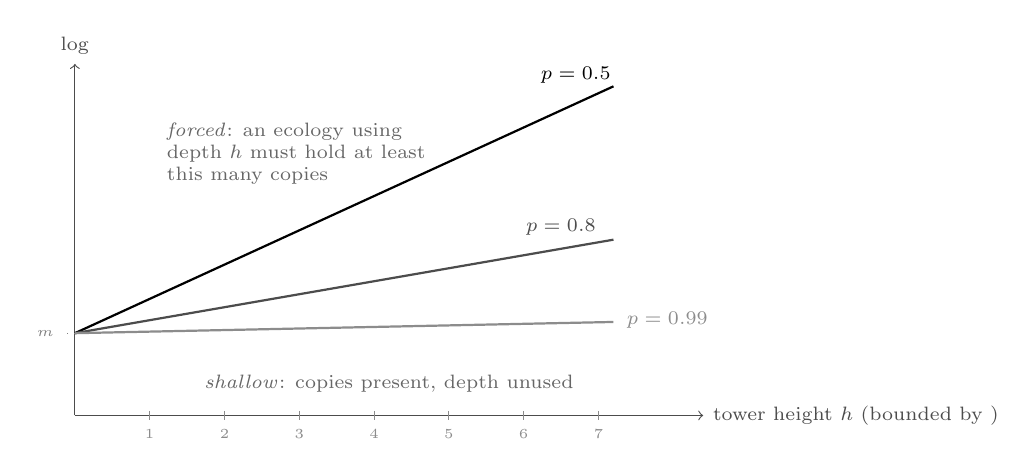
\begin{tikzpicture}[scale=0.95]
  \draw[->,black!70] (0,0) -- (8.4,0)
    node[right,font=\scriptsize] {tower height $h$ (bounded by $\AI$)};
  \draw[->,black!70] (0,0) -- (0,4.7) node[above,font=\scriptsize] {$\log \CN$};

  \foreach \x/\v in {1/1,2/2,3/3,4/4,5/5,6/6,7/7}
    \draw[black!45] (\x,0.06) -- (\x,-0.06) node[below,font=\tiny] {\v};

  \draw[thick] (0,1.1) -- (7.2,4.4);
  \node[font=\scriptsize,anchor=west] at (6.1,4.55) {$p=0.5$};
  \draw[thick,black!70] (0,1.1) -- (7.2,2.35);
  \node[font=\scriptsize,anchor=south west,black!70] at (5.9,2.28) {$p=0.8$};
  \draw[thick,black!45] (0,1.1) -- (7.2,1.25);
  \node[font=\scriptsize,anchor=west,black!45] at (7.25,1.28) {$p=0.99$};

  \node[font=\scriptsize,anchor=west,black!60,align=left] at (1.1,3.5)
    {\emph{forced}: an ecology using\\ depth $h$ must hold at least\\ this many copies};
  \node[font=\scriptsize,anchor=west,black!60,align=left] at (1.6,0.42)
    {\emph{shallow}: copies present, depth unused};

  \draw[dotted,black!50] (0,1.1) -- (-0.15,1.1) node[left,font=\tiny] {$m$};
\end{tikzpicture}
\caption{Proposition~\ref{scm:prop:frontier}. Each line is
$\log \CN = \log m + h \log(1/p)$: the copy number an ecology must hold to
use a tower of height $h$ on media of reliability $p$. The slope is set by
reliability alone.}
\label{scm:fig:frontier}
\end{figure}

\begin{remark}[What the biosignature becomes]
\label{scm:rmk:biosig}
``High assembly index and high copy number'' is, on this reading, not a
conjunction of independent findings but a point above a line whose slope
is $\log(1/p)$. The framework accordingly predicts something the bare
conjunction does not: the ratio $\log \CN / h$ should cluster near
$\log(1/p)$ for systems using their architecture and fall well below it
for systems that are merely abundant. A crystal is abundant and shallow; a
bacterium is deep and abundant in the proportion its chemistry can
sustain. If the ratio is measurable this is falsifiable, and it is
falsifiable in a way the conjunction is not. It also sharpens the joint
rise of Remark~\ref{rmk:joint-rise}: that remark says the two numbers go
up together after the phase transition, and this one says how fast.
\end{remark}

\subsection{A prediction about scarcity}

\begin{remark}[Depth goes before population]
\label{scm:rmk:shed}
Depth is priced exponentially and width linearly, so under a contraction
of resources a lineage should shed the exponentially priced axis first.
Reducing $h$ by one releases a factor $p^{-1}$ of the sampling requirement
at every stratum above the cut, together with the media, repair and engine
machinery of the level removed; reducing $\CN$ by one releases one
learner's maintenance. The first is worth vastly more per unit of
structural change. So we expect --- as an empirical matter, and stated as
an expectation rather than a theorem --- that lineages entering sustained
scarcity lose architectural levels before they lose population, and that
the reverse pattern indicates something other than resource pressure.
Regressive evolution in parasites and cave fauna is the obvious place to
look, and the obvious confound is that the same pressure removes the
selective reason for a level as well as the means to pay for it.
\end{remark}

\subsection{A worked composite: four skills, one individual, twelve of them}
\label{scm:sec:composite}

Now the numbers, carried through a mind whose skills are themselves
ecologies-as-mind, in the manner of \S\ref{com:sec:worked}. The
illustration is orca-shaped and the shape does no work beyond making the
skills memorable: a hunting skill, a skill for one's place in the pod, a
mating skill, and a skill for rearing calves. Each is a population of
mortal scientists in its own typed namespace with its own token colour;
the four are wired by engines; the whole closes over its namespace and is
an individual; and twelve such individuals form a pod, which is a
candidate individual one stratum up.

\paragraph{The generator.}
The individual's scope is
\[
  \Nsp \;=\; \mu X.\;
  \quo{\bigl( (\phi_{\mathrm{for}} \lor X) \mid
              (\phi_{\mathrm{pod}} \lor X) \mid
              (\phi_{\mathrm{mat}} \lor X) \mid
              (\phi_{\mathrm{rea}} \lor X) \bigr)},
\]
the four-predicate version of Definition~\ref{sco:def:gen}. The four
predicates are pairwise disjoint --- each skill's population is rooted at
its own quotation, by Proposition~\ref{com:prop:root} --- so the scope
parses uniquely, membership is decidable by
Proposition~\ref{sco:prop:descent}, and the floors may be added by
Proposition~\ref{scm:prop:disjointedges}.

\paragraph{Depths and populations.}
Each skill sits on media of its own reliability: the pod and rearing
skills run on internal, owned media ($p = 0.99$); hunting reaches across
the boundary into a noisy world ($p = 0.95$); mating runs across
\emph{another individual's} boundary and is worst ($p = 0.90$). Optimal
integration depth follows Proposition~\ref{eng:prop:fragile}, maximising
$Y(d)p^{d} - cd$ with $Y(d) = 100(1-2^{-d})$ and $c = 2$; the sampling
floor follows Proposition~\ref{scm:prop:sampfloor} with $m = 20$.

\begin{table}[h]
\centering
\begin{tabular}{lrrrrr}
\toprule
skill & $p$ & $d^\ast$ & net value & $\CN$ floor & separates at \\
\midrule
Forage & $0.95$ & $3$ & $69.0$ & $24$ & $4$ \\
Pod    & $0.99$ & $5$ & $82.1$ & $22$ & $2$ \\
Mate   & $0.90$ & $3$ & $57.8$ & $28$ & $3$ \\
Rear   & $0.99$ & $5$ & $82.1$ & $22$ & $3$ \\
\midrule
       &        &     &        & $96$ & \\
\bottomrule
\end{tabular}
\caption{The four skill-ecologies. ``Separates at'' is the modal depth at
which that skill's learners become distinguishable from the shared kernel
behaviour.}
\label{scm:tab:skills}
\end{table}

Note which skill is most expensive in copies. It is not the deepest; it is
the one on the worst medium. Mating costs $28$ learners to sustain depth
$3$ while the pod skill costs $22$ to sustain depth $5$, because
reliability enters the floor exponentially and depth only through the
exponent. An architecture is expensive where it is \emph{unreliable}, not
where it is deep.

\paragraph{The copy series.}
Twelve individuals, each with $96$ learners in four skill-ecologies:
\[
  \CN^{\bullet}(\text{pod}) \;=\; (1152,\; 48,\; 12,\; 1),
\]
being learners, skill-ecologies, individuals, and the pod itself. The flat
collapse is $1213$, a number that answers no question anyone would ask.
The ratios $1152 : 48 : 12 : 1$ are $24$, $4$ and $12$, and those are
respectively a sampling floor, a skill count and a group size --- three
different kinds of fact about the animal, which the collapse blends into
one meaningless total.

\paragraph{The assembly floor.}
Applying Table~\ref{scm:tab:floors} with the additivity of
Proposition~\ref{scm:prop:disjointedges}:

\begin{table}[h]
\centering
\begin{tabular}{lrl}
\toprule
component & steps & from \\
\midrule
kernel: inside, boundary, germ, stack, assay & $5$ & L1--L3, paid once \\
differentia: $d^\ast$ per skill, $3+5+3+5$   & $16$ & L4, L5 \\
wiring: joining four parts, $\lceil \log_2 4\rceil$ & $2$ & \\
engines: four, to close a cycle over four colours & $4$ & L6 \\
closure of the individual's namespace        & $1$ & L2 \\
\midrule
\textbf{floor} & $\mathbf{28}$ & \\
\midrule
same, with no kernel sharing ($5 \times 4$)  & $43$ & \\
\bottomrule
\end{tabular}
\caption{The assembly floor of the four-skill individual.}
\label{scm:tab:floor}
\end{table}

Two numbers to take from this. Sharing the kernel across the four skills
saves $15$ of $43$ steps, or $34.9\%$; and of the $28$ remaining, $16$ ---
$57.1\%$ --- are \emph{content} rather than architecture. The fractal is
cheap and the niches are expensive.

\begin{remark}[The economy runs the other way from intuition]
\label{scm:rmk:economy}
One expects a mind made of minds to be expensive because it is deep. It is
not: depth is what the fixed point gives away, since a generator that
describes one level describes all of them, and copies of a made thing are
free in assembly index. What a multi-skilled mind pays for is
\emph{differentiation} --- the distinct predicates, assays and token
colours that make hunting not-mating. Under this accounting an animal's
assembly index tracks the number of distinct niches it addresses far more
closely than the elaborateness of its architecture, and two animals of
very different apparent sophistication addressing the same number of
niches should come out close together.
\end{remark}

\paragraph{Does the whole close?}
By \S\ref{eng:S8} a region may close over its namespace exactly when its
isoperimetric ratio clears $(\varepsilon\theta/\rho)\,r$. Taking
$\theta = 0.2$, $\rho = 5$ and $\varepsilon = 1-p$ for the relevant media:
the individual, with internal media at $p = 0.99$ and two of its four
skills facing outward so that $h = 0.5$, has
$\varepsilon\theta/\rho = 4\times 10^{-4}$ and critical radius
$r^\ast = 1250$; it closes with enormous margin. The pod, whose media run
across individual boundaries at $p = 0.90$ and whose isoperimetric ratio
we take as $0.3$, has $\varepsilon\theta/\rho = 4\times 10^{-3}$ and
$r^\ast = 75$. A pod of twelve closes. An aggregation of two hundred does
not.

\begin{remark}[A critical group size, and how much to believe it]
\label{scm:rmk:groupsize}
The number $75$ is a consequence of parameters we invented, and nothing
here determines $\theta$, $\rho$ or the isoperimetric ratio of a pod. What
is not invented is the shape of the result: there is a finite size beyond
which a social aggregation cannot close over its namespace, it scales as
$\rho/(\varepsilon\theta)$, and it is set by the reliability of the media
running \emph{between} individuals rather than by anything about the
individuals. We note without pressing it that the literature on cohesive
group size in social mammals lives in this neighbourhood, and that the
framework predicts the bound should move with communication reliability
rather than with brain size. We would not want that repeated as a result.
\end{remark}

\paragraph{What a passing instrument sees.}
Finally the point of \S\ref{scm:sec:graded}, made concrete. The four
skills' learners share the kernel and separate at depths $2, 3, 3, 4$. An
observer surveying the pod's namespace at resolution $n$ reports:

\begin{table}[h]
\centering
\small
\begin{tabular}{crrl}
\toprule
resolution $n$ & kinds & largest class & \\
\midrule
$0$ & $1$ & $1152$ & everything is one kind \\
$1$ & $1$ & $1152$ & \\
$2$ & $2$ & $888$ & the pod skill separates \\
$3$ & $4$ & $336$ & mating and rearing separate \\
$\ge 4$ & $4$ & $336$ & truth \\
\bottomrule
\end{tabular}
\caption{An observer's report on the learner stratum, by resolution. Truth
is four kinds, largest class $336$.}
\label{scm:tab:observer}
\end{table}

An instrument at resolution $0$ reports a copy number $3.4$ times the
truth and a monoculture where there are four kinds; at resolution $2$ it
is still wrong by a factor of $2.6$ on the largest class. And note the
small mercy at $n = 3$: once every kind but one has been separated, the
last comes free, because what remains in the pool is a kind by
elimination. A survey therefore needs resolution equal to the
second-deepest separation, not the deepest --- a saving of exactly one
kind's worth of instrument, and the only place in this chapter where the
accounting is generous.

\section{The survey, in rholang}
\label{scm:sec:code}

Two contracts. The first decides membership in a generated scope by
descent, per Proposition~\ref{sco:prop:descent}. The second surveys a
scope and returns a copy series. Both follow the conventions of
\S\ref{gam:app:code}: a bare parameter is a name, an \texttt{@}-pattern
binds data, and a channel is passed as \texttt{*c}. Guards marked
\texttt{//!\ ideal} stand for decision procedures assumed rather than
implemented.

\begin{lstlisting}
new InScope, Split, Survey, Series, BisimN, Atom, Stratum in {

  // ---- membership by descent -------------------------------------
  // mu X . @( (phi \/ X) | (psi \/ X) ), presented as a list of
  // atomic predicates and tested by structural descent on the quote.

  contract InScope(@nm, atoms, ret) = {
    new hit in {
      Atom!(nm, *atoms, *hit) |
      for (@isAtom <- hit) {
        if (isAtom) { ret!(true) }
        else {
          // By "Unique decomposition" the split is unique, so one
          // split and two recursive calls -- no search.
          new sp in {
            Split!(nm, *sp) |
            for (@p, @q, @ok <- sp) {
              if (not ok) { ret!(false) }
              else {
                new l, r in {
                  InScope!(p, *atoms, *l) |
                  InScope!(q, *atoms, *r) |
                  for (@a <- l & @b <- r) { ret!(a and b) }
                }
              }
            }
          }
        }
      }
    }
  } |

  // Split returns the unique decomposition of a quoted parallel
  // composition.  Termination of the recursion above is exactly the
  // no-self-code theorem: p and q code strictly smaller terms.
  contract Split(@nm, ret) = {
    match *nm {
      { P | Q } => { ret!(@P, @Q, true) }        //! ideal
      _         => { ret!(Nil, Nil, false) }
    }
  } |

  // ---- the survey ------------------------------------------------
  // Visit each channel of the scope, decide n-step bisimilarity with
  // the target, and bin by stratum.  One metered rendezvous per
  // visit: this contract is where a copy number is paid for.

  contract Survey(@target, chans, @n, ret) = {
    new tally in {
      tally!({}) |
      for (@c <= chans) {                     // one visit per channel
        new b, s in {
          BisimN!(c, target, n, *b) |         //! ideal, cost kappa(n)
          Stratum!(c, *s) |
          for (@same <- b & @j <- s) {
            for (@acc <- tally) {
              if (same) { tally!(acc.set(j, acc.getOrElse(j,0) + 1)) }
              else      { tally!(acc) }
            }
          }
        }
      } |
      for (@acc <- tally) { ret!(acc) }       // the copy series
    }
  } |

  // The flat collapse, for comparison with the received definition.
  contract Series(@series, ret) = {
    ret!( series.values().fold(0, (a, b) => a + b) )
  }
}
\end{lstlisting}

\noindent
Three things the listing makes visible that the prose does not. The
recursion in \texttt{InScope} has no depth bound in its own code --- it
terminates because of a theorem about the calculus, not because of a
counter. \texttt{Survey} charges once per channel, which is what makes
affordable scope a budget question rather than a definitional one. And
\texttt{Series} exists only to throw information away; it is the received
copy number, written as the lossy projection it is.

\section{What this leaves}

Four things, and they belong with the gaps of
Chapter~\ref{sec:origins-gaps} rather than here, so they are recorded
there. The shortest statement of each: whether a non-well-founded scope
could be surveyed stratum by stratum; whether the copy series can tell a
merged composite from a merely composed one; whether affordable scope and
the individuation fixed point of Remark~\ref{eng:rem:fixpoint} have a
common solution; and what a copy number looks like once one admits that a
survey is an assay, and so has a third outcome.

There is also a connection that runs forward rather than sideways. A
learner's region is bounded by what it can pay to survey, so the
unsurveyable is not the unknowable in principle but the unaffordable in
fact --- and that is precisely the distinction
\S\ref{sec:kant-affordable} builds on when it argues that the noumenal
survives in this framework as a budget constraint rather than as a wall.
Copy number turns out to be a place where that abstraction has a number
attached: what a mind can count is bounded by what it was assembled to
resolve, and what it can survey is bounded by what it can afford to visit.
Both bounds are economic, both are movable, and neither is a limit on what
is there.

% ===================================================================
